\chapter{Resultados experimentales}

\begin{chapquote}{Platón, \textit{Alegoría de la cueva}}
\textsc{Socrates}: Imagina esto: Un grupo de personas vive en una caverna debajo de la tierra. ... Las personas han estado ahí desde pequeños, encadenados de las piernas y el cuello. ... Alguna luz, digamos de un fuego, que emite su brillo hacia ellos a sus espaldas, ... Entre el fuego y aquellos que están encadenados hay una pasarela a cierta altura. ... una pared baja ha sido contruida a lo largo de esta pasarela, como la cortina baja que alza un ventrilocuo, ... a lo largo de esta pared se pasean personas con todo tipo de cosas que la sobrepasan.

\hspace{2em}\textsc{Glaucon}: ... estos son prisioneros inusuales.

\hspace{2em}\textsc{Socrates}: Ellos son muy parecidos a nosotros los humanos...
\end{chapquote}

Se ha evaluado el algoritmo de conversión al polinomio de \textit{Zhegalkin}, en cuenta al tiempo de ejecución, usando casos de prueba para la coloración de grafos. Además de eso, se ha implementado un generador de casos a partir de instancias de grafos, aprovechando la implementación de proposiciones lógicas en \textit{Haskell} junto a una función que construye las restricciones dependiendo del número de colores con los que se intente colorear.

\section{Factores determinantes}

El tiempo de ejecución cuando se realiza la conversión a un polinomio está determinado, no solo por el número de restricciones que conforme la fórmula lógica, sino por el tamaño del arreglo de \textit{bits} para los monomios. Aun cuando sea el mismo caso de prueba, la capacidad específicada para el arreglo de \textit{bits} tiene impacto en la ejecución del algoritmo, independientemente de si se usa la \textit{GPU} o no.

Otro factor importante es la multiplicación de polinomios, cuando se multiplica un monomio por un polinomio ordenado, no se puede garantizar que el orden se mantenga. Esto implica que se deben ordenar constantemente los polinomios a medida que se van realizando las distintas operaciones. Por otro lado, la opearación de multiplicación es la que tiene mayor complejidad resultando en $O(n^2)$, como ya hemos mencionado en capítulos anteriores y ese es el punto crucial de las pruebas que se realizaron.

Un último problema importante es la tarjeta gráfica que se tuvo disponible para las pruebas, esta fue una \textit{Intel(R) HD Graphics Haswell GT2 Mobile} que viene integrada con la \textit{CPU}. La cual posee un número muy limitado de unidades de cómputo disponibles para distribuir las tareas que se delegan. Esto limita un poco el rango de pruebas pero omitiendo eso, a continuación se presentan los resultados obtenidos.

\section{Capacidad máxima de los monomios}

La capacidad máxima de los monomios se establece en conjunto con el caso de prueba que se quiera resolver, mientras el tamaño del caso sea mayor se necesita que la capacidad sea mayor. Si el número de variables es menor que la capacidad máxima entonces se estará desperdiciando un espacio de memoria que nunca tendrá impacto en el resultado final; pero si tendrá incidencia en el tiempo de ejecución.

Se realizaron pruebas donde se usaba el mismo caso de prueba pero con variaciones en la capacidad de los monomios y efectivamente el tiempo de ejecución resulta tener un incremento exponencial a medida que el arreglo de \textit{bits} es más grande. Asi que lo ideal es ajustar esta constante para que la ejecución sea la más eficiente posible dependiendo de las dimensiones del caso de prueba. En la figura \ref{fig:time} se puede ver el comportamiento del algoritmo mientras se incrementa la capacidad del monomio.

\begin{figure}[!ht]
    \centering
    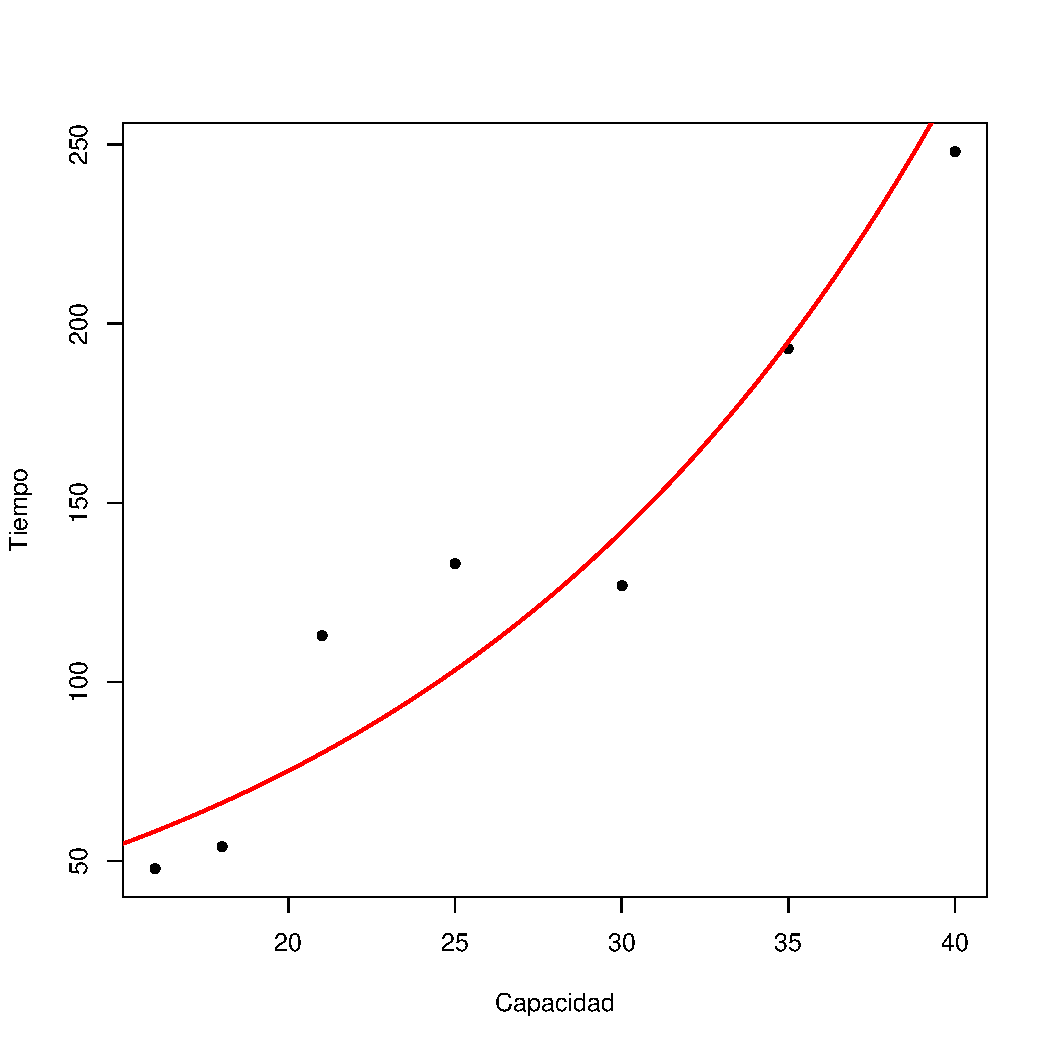
\includegraphics[width=0.7\textwidth,height=\textheight,keepaspectratio]{capacity_time.pdf}
    \caption{Comportamiento de tiempo según los monomios}
    \label{fig:time}
\end{figure}

\section{\textit{CPU vs. GPU}}

Ahora, teniendo dos versiones de la misma porción del algoritmo, una secuencial y otra en paralelo, solo quedaría ver cuál de las dos tiene mejor desempeño. Se realizaron varias pruebas en este punto, ajustando los parámetros de configuración para obtener los mejores resultados. Sorprendentemente, el tiempo de ejecución para la versión \textit{GPU} resulta tener un desempeño ligeramente peor. Esto puede deberse a varias cosas, entre ellas: la tarjeta gráfica utilizada, carga computacional para delegar tareas y recoger resultados o delegación de cómputos muy sencillos; las mismas se describen a continuación.

\subsection{Procesamiento limitado de la \textit{GPU}}

La \textit{GPU} disponible no tiene las mejores especificaciones para realizar pruebas que requieran múltiples cómputos. Dado que existe una relación entre el tipo de tarea que se le delegue a la \textit{GPU}, y la forma como son asignados estos pequeños trabajos, con la cantidad de unidades de cómputo que tenga el dispositivo.

\subsection{Delegar trabrajo tiene su precio}

Crear un contexto, cola de comandos, establecer los parámetros de una función \textit{kernel} y ejecutar ese programa tiene un costo en términos de tiempo. Por lo que sería conveniente asignar tareas que requieran más trabajo por parte de cada unidad del dispositivo. También puede incrementarse el número de trabajos delegados, cambiando la estrategia de paralelismo, pero la \textit{GPU} sigue sin tener grandes capacidades.

\subsubsection{Asignación de tareas}

En OpenCL existe un parámetro para indicar el número de elementos con los que trabajará cada unidad, es decir, cómo se distribuye el trabajo total. Por ejemplo, si se indica que cada unidad va a trabajar con una tarea a la vez del total, y este total es mayor que el número de unidades en el dispositivo, se necesitaría esperar a que se desocupe alguna unidad para asignarle una nueva tarea. Por ello, se asginan en grupos para aprovechar toda la \textit{GPU} pero si esta es limitada, y el número total de tareas es muy grande, los recursos se ven colapsados.